\chapter{Creating a basic mod (MWE)}

When developing a mod you should work in the directory \aoehomelocaldir{}.
Start by creating a folder with the same name as the mod you want to create. For this tutorial, we will create a mod that changes the background of the main menu: we will name such a folder \dquote{carcassone-menu}.

For this very reason we need to put the background image (in this case the one shown in \figref{fig:carcassonne})

\begin{figure}[ht]
    \centering
    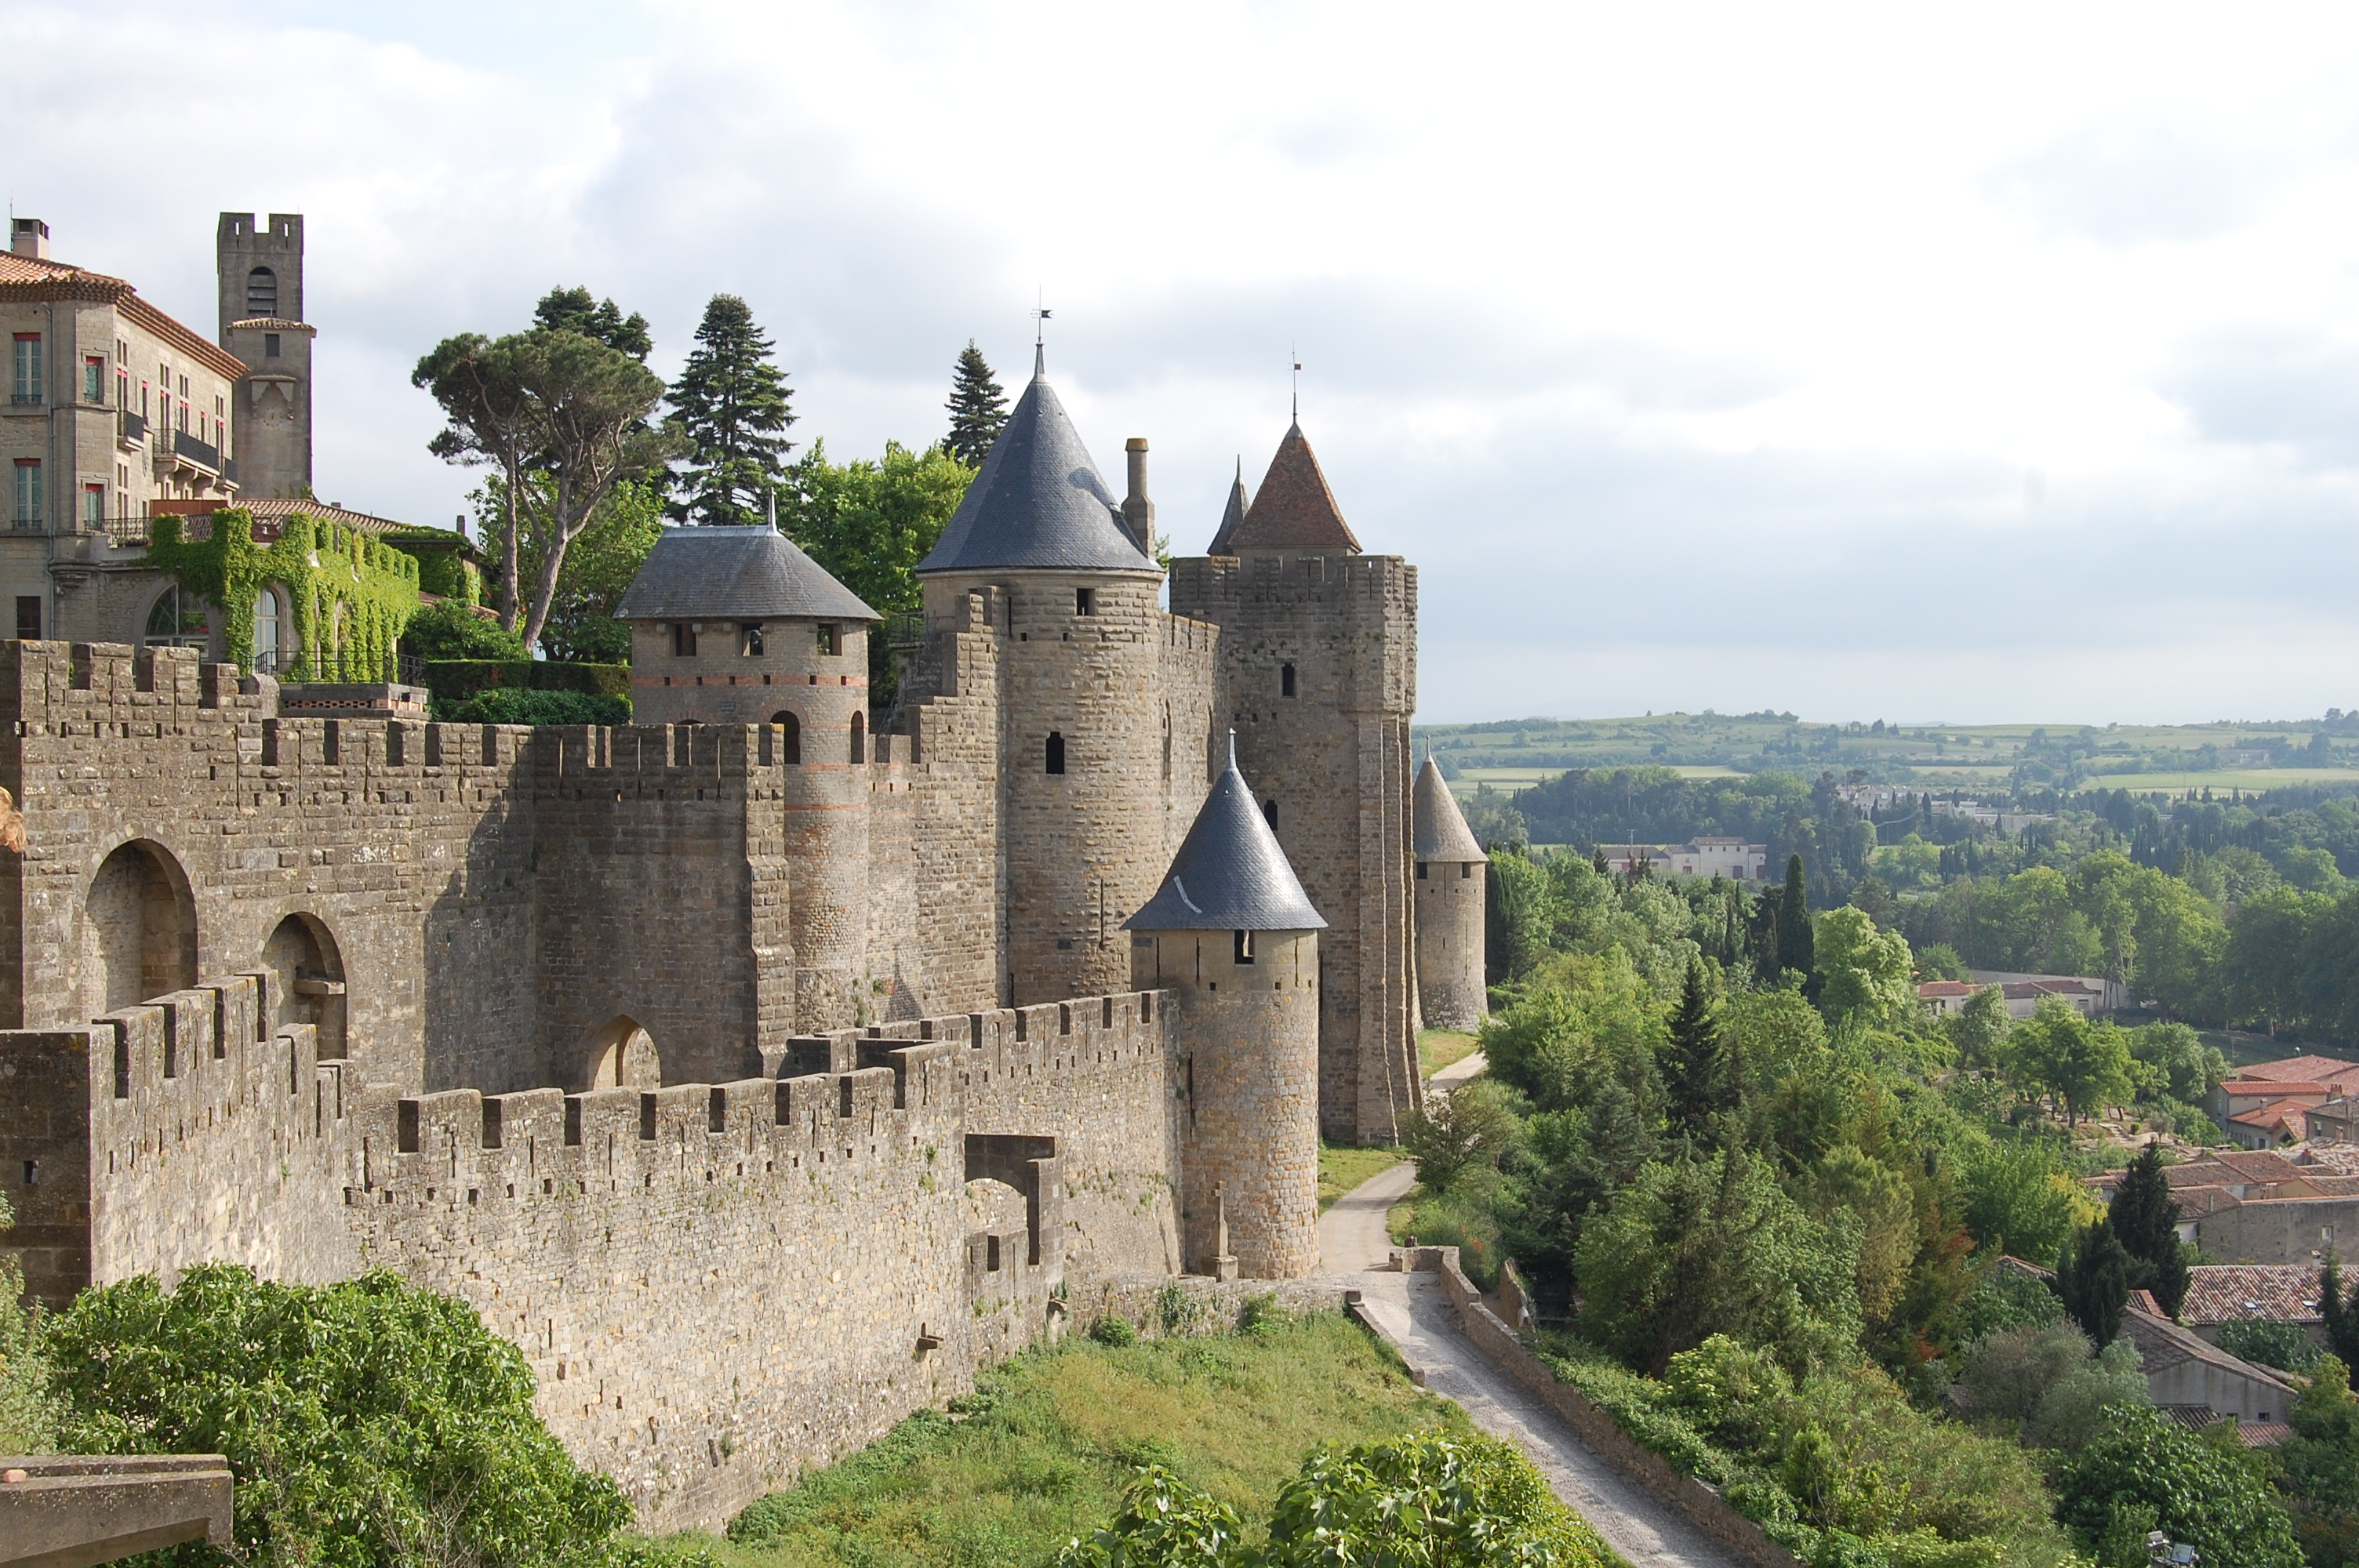
\includegraphics[width=1.0\textwidth]{src/images/carcassonne}
    \caption{Image to put as background}
    \label{fig:carcassonne}
\end{figure}

As shown in the Appendix \ref{chp:semantics}, the background image is specified (relative to \aoeexedir{}) in \code{widgetui/textures/backgrounds/mainmenu\_bg.dds}.
Hence, in the \dquote{carcassone-menu} folder, you need to create the subfolder \code{widgetui/textures/backgrounds/mainmenu\_bg}; then you need to put the Carcassone image, name it \dquote{mainmenu\_bg} (ensure that the image follows the \acrref{DDS} extension).

\lstinputlisting[label=verb3,caption={Carcassonne mod layout}, float, frame=ht]{src/codes/carcassonne-mod-layout.txt}

Aside the folders you have just created, you need two additional files that represents mod metadata. Both files needs to be put in \dquote{carcassone-menu} folders. The first is \code{thumbnail.jpg}, which is a jpg format that is shown when browsing the mods. The other metadata file is call \dquote{info.json} (an example is shown in \lstref{verb4}): it is a json containing 3 values:
\begin{itemize}
    \item Author: name of the author of this mod;
    \item Description: a description of the mod;
    \item Title: title to show of the mod;
\end{itemize}

If the developer puts other fields in this json, they will be automatically removed. Any formatting will be overwritten as well.
All the metadata is shown in the right panel of the mod browsing window (in \aoe{} program, Mods section). Additional files in \aoehomelocaldir{} mod will be left in the folder

\lstinputlisting[language={json},label=verb4,caption={Carcassonne mod layout}, float, frame=ht]{src/codes/carcassonne-mod-layout.txt}

The thumbnail can have any dimensions, although 400x150-ish dimensions may be preferred.
After this operation, open \aoe{}, go to the mods, specifically to \dquote{My Mods}. If you click \dquote{Import My Mods} \aoe{} will search into the \aoehomelocaldir{} for compliant mods. You should see the new mods (as shown in \figref{fig:mymods}).

\begin{figure}[ht]
    \centering
    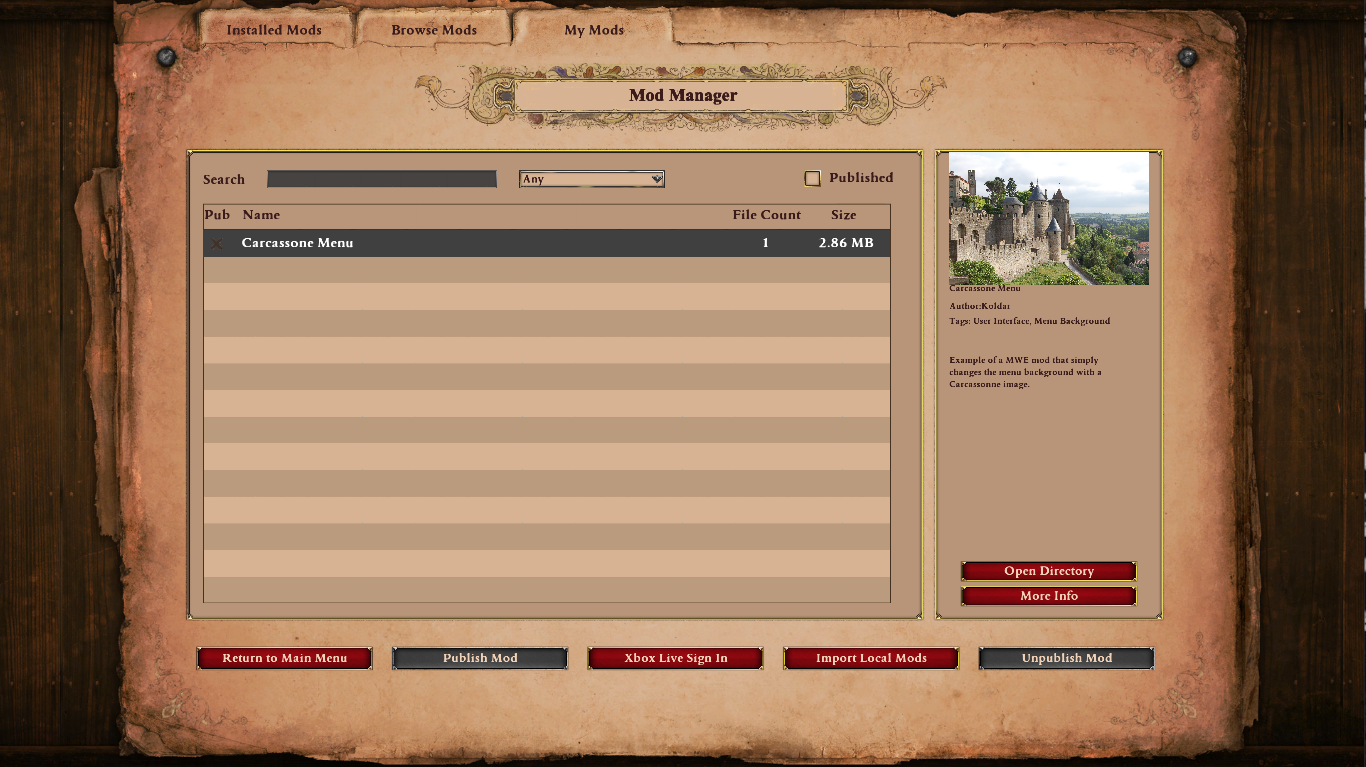
\includegraphics[width=1.0\textwidth]{src/images/mymods}
    \caption{My mods window}
    \label{fig:mymods}
\end{figure}

The image in the background will be clipped. \dquote{mod-status.json} will be automatically updated.

\begin{warning}
    If \code{thumbnail.jpg} is not present, a default image will be put instead. If \code{info.json} is absent, default values will be put: at the moment of writing, the author is set to \dquote{Unpublished}, description to \dquote{No Description} and name as the same folder as the mod root dir. If \dquote{info.json} content is lacking one of those 3 fields, \aoe{} will automatically fill the missing ones.
\end{warning}

In the mod window, if you select the \dquote{carcassonne-menu} you click \dquote{More Info}. If you click this, \aoe{} will automatically open the browser at the \acrref{URL} \url{https://www.ageofempires.com/mods/details/XYZ} where $XYZ$ is the WorkShop Id of the mod. If \aoe{} fails to load the mods, you can \textit{debugging} the mod by make changes the mod in \aoehomelocaldir{} and click \dquote{Import Local Mods} button.

\section{Publish mod}

It is now time to publish the mod. In this way the mod can be automatically downloaded by other client if it is required in a lobby game. In order to publish the mod you need to visit \url{www.ageofempires.com} and sign in with a \textit{XBox Live Account} (Logging with the Steam one is not enough). 

Choose the mod you want to publish and zip the content of the entire mod folder (\ie{} the one containing the file \dquote{info.json} and \dquote{thumbnail.jpg}): this means that if you open the zip file, you will immediately find at the top level the files \dquote{info.json} and \dquote{thumbnail.jpg};\footnote{With \code{7-Zip}, if you right-click the zip and you \dquote{Open} it, you should find such files inside the windows that has just appeared.} then, visit \url{https://www.ageofempires.com/mods/create/} and fill the form with all the required information and finally submit. After some time, you should have published your mode.

Alternatively, you can sign-in inside \aoe{} with you \textit{XBox Live Account}. Then, you can visit te \dquote{My Mods} tab and click on \dquote{Publish Mod} or update when you want to publish a new version of the same mod.
